\documentclass[twoside]{book}

% Packages required by doxygen
\usepackage{calc}
\usepackage{doxygen}
\usepackage{graphicx}
\usepackage[utf8]{inputenc}
\usepackage{makeidx}
\usepackage{multicol}
\usepackage{multirow}
\usepackage{textcomp}
\usepackage[table]{xcolor}

% Font selection
\usepackage[T1]{fontenc}
\usepackage{mathptmx}
\usepackage[scaled=.90]{helvet}
\usepackage{courier}
\usepackage{amssymb}
\usepackage{sectsty}
\renewcommand{\familydefault}{\sfdefault}
\allsectionsfont{%
  \fontseries{bc}\selectfont%
  \color{darkgray}%
}
\renewcommand{\DoxyLabelFont}{%
  \fontseries{bc}\selectfont%
  \color{darkgray}%
}

% Page & text layout
\usepackage{geometry}
\geometry{%
  a4paper,%
  top=2.5cm,%
  bottom=2.5cm,%
  left=2.5cm,%
  right=2.5cm%
}
\tolerance=750
\hfuzz=15pt
\hbadness=750
\setlength{\emergencystretch}{15pt}
\setlength{\parindent}{0cm}
\setlength{\parskip}{0.2cm}
\makeatletter
\renewcommand{\paragraph}{%
  \@startsection{paragraph}{4}{0ex}{-1.0ex}{1.0ex}{%
    \normalfont\normalsize\bfseries\SS@parafont%
  }%
}
\renewcommand{\subparagraph}{%
  \@startsection{subparagraph}{5}{0ex}{-1.0ex}{1.0ex}{%
    \normalfont\normalsize\bfseries\SS@subparafont%
  }%
}
\makeatother

% Headers & footers
\usepackage{fancyhdr}
\pagestyle{fancyplain}
\fancyhead[LE]{\fancyplain{}{\bfseries\thepage}}
\fancyhead[CE]{\fancyplain{}{}}
\fancyhead[RE]{\fancyplain{}{\bfseries\leftmark}}
\fancyhead[LO]{\fancyplain{}{\bfseries\rightmark}}
\fancyhead[CO]{\fancyplain{}{}}
\fancyhead[RO]{\fancyplain{}{\bfseries\thepage}}
\fancyfoot[LE]{\fancyplain{}{}}
\fancyfoot[CE]{\fancyplain{}{}}
\fancyfoot[RE]{\fancyplain{}{\bfseries\scriptsize Generated on Thu Mar 24 2016 19\-:51\-:00 for rpg tools (\-Python) by Doxygen }}
\fancyfoot[LO]{\fancyplain{}{\bfseries\scriptsize Generated on Thu Mar 24 2016 19\-:51\-:00 for rpg tools (\-Python) by Doxygen }}
\fancyfoot[CO]{\fancyplain{}{}}
\fancyfoot[RO]{\fancyplain{}{}}
\renewcommand{\footrulewidth}{0.4pt}
\renewcommand{\chaptermark}[1]{%
  \markboth{#1}{}%
}
\renewcommand{\sectionmark}[1]{%
  \markright{\thesection\ #1}%
}

% Indices & bibliography
\usepackage{natbib}
\usepackage[titles]{tocloft}
\setcounter{tocdepth}{3}
\setcounter{secnumdepth}{5}
\makeindex

% Hyperlinks (required, but should be loaded last)
\usepackage{ifpdf}
\ifpdf
  \usepackage[pdftex,pagebackref=true]{hyperref}
\else
  \usepackage[ps2pdf,pagebackref=true]{hyperref}
\fi
\hypersetup{%
  colorlinks=true,%
  linkcolor=blue,%
  citecolor=blue,%
  unicode%
}

% Custom commands
\newcommand{\clearemptydoublepage}{%
  \newpage{\pagestyle{empty}\cleardoublepage}%
}


%===== C O N T E N T S =====

\begin{document}

% Titlepage & ToC
\hypersetup{pageanchor=false}
\pagenumbering{roman}
\begin{titlepage}
\vspace*{7cm}
\begin{center}%
{\Large rpg tools (Python) \\[1ex]\large 1.\-0a }\\
\vspace*{1cm}
{\large Generated by Doxygen 1.8.6}\\
\vspace*{0.5cm}
{\small Thu Mar 24 2016 19:51:00}\\
\end{center}
\end{titlepage}
\clearemptydoublepage
\tableofcontents
\clearemptydoublepage
\pagenumbering{arabic}
\hypersetup{pageanchor=true}

%--- Begin generated contents ---
\chapter{Todo List}
\label{todo}
\hypertarget{todo}{}

\begin{DoxyRefList}
\item[\label{todo__todo000001}%
\hypertarget{todo__todo000001}{}%
File \hyperlink{Backpack_8py}{Backpack.py} ]Modul\-: reading and interpreting mysql configuration 

Modul\-: create intial mysql db 

Modul\-: insert, update and read data from db 

Modul\-: saves extracted data as P\-D\-F  
\item[\label{todo__todo000002}%
\hypertarget{todo__todo000002}{}%
Global \hyperlink{classcalc__ep_1_1MainWindow_a784d15d1157ea5b181c63d73daa3fc5e}{Main\-Window.help\-Handbook} ]this needs to be implemented  
\item[\label{todo__todo000003}%
\hypertarget{todo__todo000003}{}%
Global \hyperlink{classgui_1_1window_1_1MainWindow_a784d15d1157ea5b181c63d73daa3fc5e}{Main\-Window.help\-Handbook} ]this needs to be implemented  
\item[\label{todo__todo000011}%
\hypertarget{todo__todo000011}{}%
Global \hyperlink{classgui_1_1window2_1_1MainWindow_a784d15d1157ea5b181c63d73daa3fc5e}{Main\-Window.help\-Handbook} ]this needs to be implemented  
\item[\label{todo__todo000024}%
\hypertarget{todo__todo000024}{}%
Global \hyperlink{classgui_1_1window3_1_1MenuWin_ab66f1da42371ac6f08a9817adf59a38e}{Menu\-Win.add\-Help} ]\-: add additional help contexts -\/ maybe even a real {\itshape context} {\itshape help}  
\item[\label{todo__todo000026}%
\hypertarget{todo__todo000026}{}%
Global \hyperlink{classgui_1_1window3_1_1MenuWin_a4b810e6adc7d147eaa8edb45dd5891ca}{Menu\-Win.context\-Help} ]\-: Implement a context help method  
\item[\label{todo__todo000025}%
\hypertarget{todo__todo000025}{}%
Global \hyperlink{classgui_1_1window3_1_1MenuWin_a2e91f76cce6e9b7a03830202f45aecf0}{Menu\-Win.first\-Steps} ]\-: implement this help method 

\-: write the first step howtos...  
\item[\label{todo__todo000028}%
\hypertarget{todo__todo000028}{}%
Namespace \hyperlink{namespacetoolbox}{toolbox} ]Create the modules for Python 3.\-x  
\item[\label{todo__todo000030}%
\hypertarget{todo__todo000030}{}%
File \hyperlink{xmlbox_8py}{xmlbox.py} ]There have be a clean out and a unifying of dictionary keys... 
\end{DoxyRefList}
\chapter{Namespace Index}
\section{Namespace List}
Here is a list of all documented namespaces with brief descriptions\-:\begin{DoxyCompactList}
\item\contentsline{section}{\hyperlink{namespacecalc__ep}{calc\-\_\-ep} \\*This is a little tool for calculating E\-Ps for M\-E\-R\-S/\-R\-M }{\pageref{namespacecalc__ep}}{}
\item\contentsline{section}{\hyperlink{namespacegui}{gui} \\*Classes and stuff for the G\-U\-I }{\pageref{namespacegui}}{}
\item\contentsline{section}{\hyperlink{namespacegui_1_1window}{gui.\-window} }{\pageref{namespacegui_1_1window}}{}
\item\contentsline{section}{\hyperlink{namespacerpgtoolbox}{rpgtoolbox} \\*D\-Efinitions for E\-P-\/\-Calculator }{\pageref{namespacerpgtoolbox}}{}
\item\contentsline{section}{\hyperlink{namespacerpgtoolbox_1_1rpgtools}{rpgtoolbox.\-rpgtools} \\*R\-P\-G helpful functions This module contains some helpful functions for role-\/playing games like\-: }{\pageref{namespacerpgtoolbox_1_1rpgtools}}{}
\item\contentsline{section}{\hyperlink{namespacerpgToolDefinitions}{rpg\-Tool\-Definitions} \\*Help functions for rpg }{\pageref{namespacerpgToolDefinitions}}{}
\item\contentsline{section}{\hyperlink{namespacerpgToolDefinitions_1_1epcalcdefs}{rpg\-Tool\-Definitions.\-epcalcdefs} \\*D\-Efinitions for E\-P-\/\-Calculator }{\pageref{namespacerpgToolDefinitions_1_1epcalcdefs}}{}
\item\contentsline{section}{\hyperlink{namespacetoolbox}{toolbox} \\*A toolbox for the adamant xml profile generator }{\pageref{namespacetoolbox}}{}
\end{DoxyCompactList}

\chapter{Hierarchical Index}
\section{Class Hierarchy}
This inheritance list is sorted roughly, but not completely, alphabetically\-:\begin{DoxyCompactList}
\item \contentsline{section}{adamant\-X\-M\-L}{\pageref{classrpgtoolbox_1_1errbox_1_1adamantXML}}{}
\item \contentsline{section}{adamant\-X\-M\-L}{\pageref{classrpgToolDefinitions_1_1toolbox_1_1errbox_1_1adamantXML}}{}
\item \contentsline{section}{Auto\-Scrollbar}{\pageref{classgui_1_1winhelper_1_1AutoScrollbar}}{}
\item \contentsline{section}{blank\-Window}{\pageref{classgui_1_1window_1_1blankWindow}}{}
\begin{DoxyCompactList}
\item \contentsline{section}{Main\-Window}{\pageref{classcalc__ep_1_1MainWindow}}{}
\item \contentsline{section}{attrib\-Win}{\pageref{classgui_1_1window_1_1attribWin}}{}
\item \contentsline{section}{conf\-Window}{\pageref{classgui_1_1window_1_1confWindow}}{}
\item \contentsline{section}{input\-Win}{\pageref{classgui_1_1window_1_1inputWin}}{}
\item \contentsline{section}{Main\-Window}{\pageref{classgui_1_1window_1_1MainWindow}}{}
\item \contentsline{section}{meta\-Win}{\pageref{classgui_1_1window_1_1metaWin}}{}
\end{DoxyCompactList}
\item \contentsline{section}{blank\-Window}{\pageref{classgui_1_1window2_1_1blankWindow}}{}
\begin{DoxyCompactList}
\item \contentsline{section}{attrib\-Meta\-Win}{\pageref{classgui_1_1window2_1_1attribMetaWin}}{}
\item \contentsline{section}{attrib\-Win}{\pageref{classgui_1_1window2_1_1attribWin}}{}
\item \contentsline{section}{conf\-Window}{\pageref{classgui_1_1window2_1_1confWindow}}{}
\item \contentsline{section}{connect\-Elem}{\pageref{classgui_1_1window2_1_1connectElem}}{}
\item \contentsline{section}{input\-Win}{\pageref{classgui_1_1window2_1_1inputWin}}{}
\item \contentsline{section}{Main\-Window}{\pageref{classgui_1_1window2_1_1MainWindow}}{}
\item \contentsline{section}{meta\-Win}{\pageref{classgui_1_1window2_1_1metaWin}}{}
\end{DoxyCompactList}
\item \contentsline{section}{chk\-Cfg}{\pageref{classrpgtoolbox_1_1confbox_1_1chkCfg}}{}
\item \contentsline{section}{chk\-Cfg}{\pageref{classrpgToolDefinitions_1_1toolbox_1_1confbox_1_1chkCfg}}{}
\item \contentsline{section}{draw\-Tree}{\pageref{classgui_1_1window2_1_1drawTree}}{}
\item \contentsline{section}{handle\-X\-M\-L}{\pageref{classrpgToolDefinitions_1_1toolbox_1_1xmltools_1_1handleXML}}{}
\item \contentsline{section}{Info\-Canvas}{\pageref{classgui_1_1winhelper_1_1InfoCanvas}}{}
\item \contentsline{section}{Magic}{\pageref{classrpgToolDefinitions_1_1MERSTables_1_1Magic}}{}
\item \contentsline{section}{Menu\-Win}{\pageref{classgui_1_1window3_1_1MenuWin}}{}
\item \contentsline{section}{message\-Window}{\pageref{classgui_1_1window_1_1messageWindow}}{}
\item \contentsline{section}{message\-Window}{\pageref{classgui_1_1window2_1_1messageWindow}}{}
\item \contentsline{section}{message\-Window}{\pageref{classgui_1_1window3_1_1messageWindow}}{}
\item \contentsline{section}{My\-Class}{\pageref{classrpgToolDefinitions_1_1RMTables_1_1MyClass}}{}
\end{DoxyCompactList}

\chapter{Data Structure Index}
\section{Data Structures}
Here are the data structures with brief descriptions\-:\begin{DoxyCompactList}
\item\contentsline{section}{\hyperlink{classrpgtoolbox_1_1errbox_1_1adamantXML}{adamant\-X\-M\-L} \\*Objects of this class will be raised in case of errors with X\-M\-L files used for A\-Da\-Mant }{\pageref{classrpgtoolbox_1_1errbox_1_1adamantXML}}{}
\item\contentsline{section}{\hyperlink{classrpgToolDefinitions_1_1toolbox_1_1errbox_1_1adamantXML}{adamant\-X\-M\-L} \\*Objects of this class will be raised in case of errors with X\-M\-L files used for A\-Da\-Mant }{\pageref{classrpgToolDefinitions_1_1toolbox_1_1errbox_1_1adamantXML}}{}
\item\contentsline{section}{\hyperlink{classgui_1_1window2_1_1attribMetaWin}{attrib\-Meta\-Win} \\*This opens a window for setting the attributes of meta data fields }{\pageref{classgui_1_1window2_1_1attribMetaWin}}{}
\item\contentsline{section}{\hyperlink{classgui_1_1window_1_1attribWin}{attrib\-Win} \\*This generates a window where attributes can be added to chosen elements of structure }{\pageref{classgui_1_1window_1_1attribWin}}{}
\item\contentsline{section}{\hyperlink{classgui_1_1window2_1_1attribWin}{attrib\-Win} \\*This generates a window where attributes can be added to chosen elements of structure }{\pageref{classgui_1_1window2_1_1attribWin}}{}
\item\contentsline{section}{\hyperlink{classgui_1_1winhelper_1_1AutoScrollbar}{Auto\-Scrollbar} \\*A scrollbar that hides itself if it's not needed }{\pageref{classgui_1_1winhelper_1_1AutoScrollbar}}{}
\item\contentsline{section}{\hyperlink{classgui_1_1window_1_1blankWindow}{blank\-Window} \\*A simple window class with a not filled menu bar }{\pageref{classgui_1_1window_1_1blankWindow}}{}
\item\contentsline{section}{\hyperlink{classgui_1_1window2_1_1blankWindow}{blank\-Window} \\*A simple window class with a not filled menu bar }{\pageref{classgui_1_1window2_1_1blankWindow}}{}
\item\contentsline{section}{\hyperlink{classrpgtoolbox_1_1confbox_1_1chkCfg}{chk\-Cfg} \\*These Objects reads out a given config file and store the content of the configuration in a dictionary }{\pageref{classrpgtoolbox_1_1confbox_1_1chkCfg}}{}
\item\contentsline{section}{\hyperlink{classrpgToolDefinitions_1_1toolbox_1_1confbox_1_1chkCfg}{chk\-Cfg} \\*These Objects reads out a given config file and store the content of the configuration in a dictionary }{\pageref{classrpgToolDefinitions_1_1toolbox_1_1confbox_1_1chkCfg}}{}
\item\contentsline{section}{\hyperlink{classgui_1_1window2_1_1confWindow}{conf\-Window} \\*This class builds a window for selecting and saving options of A\-Da\-Man\-T }{\pageref{classgui_1_1window2_1_1confWindow}}{}
\item\contentsline{section}{\hyperlink{classgui_1_1window_1_1confWindow}{conf\-Window} \\*This class builds a window for selecting and saving options of A\-Da\-Man\-T }{\pageref{classgui_1_1window_1_1confWindow}}{}
\item\contentsline{section}{\hyperlink{classgui_1_1window2_1_1connectElem}{connect\-Elem} \\*This creates a window to connect elements of structure logically }{\pageref{classgui_1_1window2_1_1connectElem}}{}
\item\contentsline{section}{\hyperlink{classgui_1_1window2_1_1drawTree}{draw\-Tree} \\*This class creates an object to draw a graph of a tree structure (in a dictionary) }{\pageref{classgui_1_1window2_1_1drawTree}}{}
\item\contentsline{section}{\hyperlink{classrpgToolDefinitions_1_1toolbox_1_1xmltools_1_1handleXML}{handle\-X\-M\-L} \\*This class offers methods to convert dictionaries to X\-M\-L and back }{\pageref{classrpgToolDefinitions_1_1toolbox_1_1xmltools_1_1handleXML}}{}
\item\contentsline{section}{\hyperlink{classgui_1_1winhelper_1_1InfoCanvas}{Info\-Canvas} \\*A Canvas-\/widget that holds a scrollable Message-\/widget }{\pageref{classgui_1_1winhelper_1_1InfoCanvas}}{}
\item\contentsline{section}{\hyperlink{classgui_1_1window_1_1inputWin}{input\-Win} \\*Objects of this class type are windows for input the wanted data structure }{\pageref{classgui_1_1window_1_1inputWin}}{}
\item\contentsline{section}{\hyperlink{classgui_1_1window2_1_1inputWin}{input\-Win} \\*Objects of this class type are windows for input the wanted data structure }{\pageref{classgui_1_1window2_1_1inputWin}}{}
\item\contentsline{section}{\hyperlink{classrpgToolDefinitions_1_1MERSTables_1_1Magic}{Magic} \\*Classdocs }{\pageref{classrpgToolDefinitions_1_1MERSTables_1_1Magic}}{}
\item\contentsline{section}{\hyperlink{classgui_1_1window_1_1MainWindow}{Main\-Window} \\*This is the class for the main window object }{\pageref{classgui_1_1window_1_1MainWindow}}{}
\item\contentsline{section}{\hyperlink{classcalc__ep_1_1MainWindow}{Main\-Window} \\*This is the class for the main window object }{\pageref{classcalc__ep_1_1MainWindow}}{}
\item\contentsline{section}{\hyperlink{classgui_1_1window2_1_1MainWindow}{Main\-Window} \\*This is the class for the main window object }{\pageref{classgui_1_1window2_1_1MainWindow}}{}
\item\contentsline{section}{\hyperlink{classgui_1_1window3_1_1MenuWin}{Menu\-Win} \\*Master class for all windows using menus }{\pageref{classgui_1_1window3_1_1MenuWin}}{}
\item\contentsline{section}{\hyperlink{classgui_1_1window_1_1messageWindow}{message\-Window} \\*A class to build a message window containing version, author and email on default }{\pageref{classgui_1_1window_1_1messageWindow}}{}
\item\contentsline{section}{\hyperlink{classgui_1_1window2_1_1messageWindow}{message\-Window} \\*A class to build a message window containing version, author and email on default }{\pageref{classgui_1_1window2_1_1messageWindow}}{}
\item\contentsline{section}{\hyperlink{classgui_1_1window3_1_1messageWindow}{message\-Window} \\*A class to build a message window containing version, author and email on default }{\pageref{classgui_1_1window3_1_1messageWindow}}{}
\item\contentsline{section}{\hyperlink{classgui_1_1window_1_1metaWin}{meta\-Win} \\*Creates a window for generating meta data fields }{\pageref{classgui_1_1window_1_1metaWin}}{}
\item\contentsline{section}{\hyperlink{classgui_1_1window2_1_1metaWin}{meta\-Win} \\*Creates a window for generating meta data fields }{\pageref{classgui_1_1window2_1_1metaWin}}{}
\item\contentsline{section}{\hyperlink{classrpgToolDefinitions_1_1RMTables_1_1MyClass}{My\-Class} \\*Created on 13.\-12.\-2015 }{\pageref{classrpgToolDefinitions_1_1RMTables_1_1MyClass}}{}
\end{DoxyCompactList}

\chapter{File Index}
\section{\-File \-List}
\-Here is a list of all documented files with brief descriptions\-:\begin{DoxyCompactList}
\item\contentsline{section}{\hyperlink{language_8py}{language.\-py} }{\pageref{language_8py}}{}
\item\contentsline{section}{\hyperlink{logtools_8py}{logtools.\-py} }{\pageref{logtools_8py}}{}
\item\contentsline{section}{\hyperlink{ostools_8py}{ostools.\-py} }{\pageref{ostools_8py}}{}
\end{DoxyCompactList}

\chapter{Namespace Documentation}
\input{namespacecalc__ep}
\hypertarget{namespacegui}{\section{gui Namespace Reference}
\label{namespacegui}\index{gui@{gui}}
}


Classes and stuff for the G\-U\-I.  


\subsection*{Namespaces}
\begin{DoxyCompactItemize}
\item 
\hyperlink{namespacegui_1_1window}{window}
\end{DoxyCompactItemize}
\subsection*{Functions}
\begin{DoxyCompactItemize}
\item 
def \hyperlink{namespacegui_a12480cf412a0cd57703e77e105709a9a}{check\-Version}
\begin{DoxyCompactList}\small\item\em This function checks out the installed (and used) Python version. \end{DoxyCompactList}\end{DoxyCompactItemize}


\subsection{Detailed Description}
Classes and stuff for the G\-U\-I. this toolbox consist of functions and classes for creating a G\-U\-I. They are used by the main module.

\begin{DoxyAuthor}{Author}
Marcus Schwamberger  \href{mailto:mongol@nld.ds}{\tt mongol@nld.\-ds} mpg.\-de 
\end{DoxyAuthor}
\begin{DoxyDate}{Date}
(c) 2012 
\end{DoxyDate}
\begin{DoxyVersion}{Version}
0.\-1 alpha 
\end{DoxyVersion}


\subsection{Function Documentation}
\hypertarget{namespacegui_a12480cf412a0cd57703e77e105709a9a}{\index{gui@{gui}!check\-Version@{check\-Version}}
\index{check\-Version@{check\-Version}!gui@{gui}}
\subsubsection[{check\-Version}]{\setlength{\rightskip}{0pt plus 5cm}def gui.\-check\-Version (
\begin{DoxyParamCaption}
{}
\end{DoxyParamCaption}
)}}\label{namespacegui_a12480cf412a0cd57703e77e105709a9a}


This function checks out the installed (and used) Python version. 

The A\-X\-G is compatible to version 2.\-6+ or 3.\-2+ \begin{DoxyReturn}{Returns}
main version number (2/3) or error (1) 
\end{DoxyReturn}

\input{namespacegui_1_1window}
\input{namespacerpgtoolbox}
\input{namespacerpgtoolbox_1_1rpgtools}
\input{namespacerpgToolDefinitions}
\input{namespacerpgToolDefinitions_1_1epcalcdefs}
\hypertarget{namespacetoolbox}{\section{toolbox Namespace Reference}
\label{namespacetoolbox}\index{toolbox@{toolbox}}
}


A toolbox for the adamant xml profile generator.  




\subsection{Detailed Description}
A toolbox for the adamant xml profile generator. A toolbox of things to handle config files.

This toolbox consist of functions and classes which are used by the main module and keep the code clean and readable. All this functions and classes are meant as 'helper tools'.

\begin{DoxyAuthor}{Author}
Marcus Schwamberger  \href{mailto:marcus@lederzeug.de}{\tt marcus@lederzeug.\-de} 
\end{DoxyAuthor}
\begin{DoxyDate}{Date}
(c) 2012 
\end{DoxyDate}
\begin{DoxyVersion}{Version}
0.\-3 alpha
\end{DoxyVersion}
\begin{DoxyRefDesc}{Todo}
\item[\hyperlink{todo__todo000028}{Todo}]Create the modules for Python 3.\-x \end{DoxyRefDesc}


\begin{DoxyAuthor}{Author}
Marcus Schwamberger 
\end{DoxyAuthor}
\begin{DoxyDate}{Date}
(c) 2012 
\end{DoxyDate}
\begin{DoxyVersion}{Version}
0.\-5.\-2 alpha  \href{mailto:marcus@lederzeug.de}{\tt marcus@lederzeug.\-de} 
\end{DoxyVersion}

\chapter{Data Structure Documentation}
\input{classrpgtoolbox_1_1errbox_1_1adamantXML}
\input{classrpgToolDefinitions_1_1toolbox_1_1errbox_1_1adamantXML}
\hypertarget{classgui_1_1window2_1_1attribMetaWin}{\section{attrib\-Meta\-Win Class Reference}
\label{classgui_1_1window2_1_1attribMetaWin}\index{attrib\-Meta\-Win@{attrib\-Meta\-Win}}
}


This opens a window for setting the attributes of meta data fields.  




Inheritance diagram for attrib\-Meta\-Win\-:\nopagebreak
\begin{figure}[H]
\begin{center}
\leavevmode
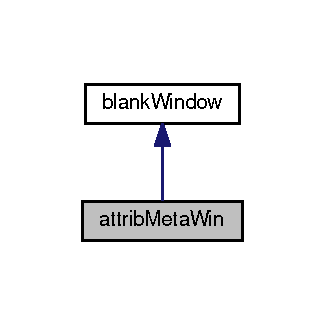
\includegraphics[width=156pt]{classgui_1_1window2_1_1attribMetaWin__inherit__graph}
\end{center}
\end{figure}


Collaboration diagram for attrib\-Meta\-Win\-:\nopagebreak
\begin{figure}[H]
\begin{center}
\leavevmode
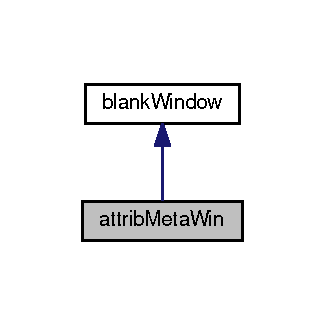
\includegraphics[width=156pt]{classgui_1_1window2_1_1attribMetaWin__coll__graph}
\end{center}
\end{figure}
\subsection*{Public Member Functions}
\begin{DoxyCompactItemize}
\item 
\hypertarget{classgui_1_1window2_1_1attribMetaWin_a615f3073891733337c33f599f89ec7ef}{def \hyperlink{classgui_1_1window2_1_1attribMetaWin_a615f3073891733337c33f599f89ec7ef}{notdoneyet}}\label{classgui_1_1window2_1_1attribMetaWin_a615f3073891733337c33f599f89ec7ef}

\begin{DoxyCompactList}\small\item\em Most important dummy method! \end{DoxyCompactList}\end{DoxyCompactItemize}


\subsection{Detailed Description}
This opens a window for setting the attributes of meta data fields. 


\begin{DoxyParams}{Parameters}
{\em lang} & used display language \\
\hline
{\em meta} & dictionary which holds the meta data field structure \\
\hline
{\em fn\-\_\-meta} & file name of meta data field's X\-M\-L file \\
\hline
{\em fn\-\_\-struc} & filename of structure element's X\-M\-L file \\
\hline
{\em storepath} & path where to store the file. If not set it is the home directory of the user. \\
\hline
\end{DoxyParams}


The documentation for this class was generated from the following file\-:\begin{DoxyCompactItemize}
\item 
\hyperlink{window2_8py}{window2.\-py}\end{DoxyCompactItemize}

\input{classgui_1_1window_1_1attribWin}
\hypertarget{classgui_1_1window2_1_1attribWin}{\section{attrib\-Win Class Reference}
\label{classgui_1_1window2_1_1attribWin}\index{attrib\-Win@{attrib\-Win}}
}


This generates a window where attributes can be added to chosen elements of structure.  




Inheritance diagram for attrib\-Win\-:\nopagebreak
\begin{figure}[H]
\begin{center}
\leavevmode
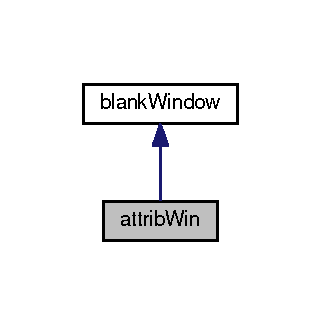
\includegraphics[width=154pt]{classgui_1_1window2_1_1attribWin__inherit__graph}
\end{center}
\end{figure}


Collaboration diagram for attrib\-Win\-:\nopagebreak
\begin{figure}[H]
\begin{center}
\leavevmode
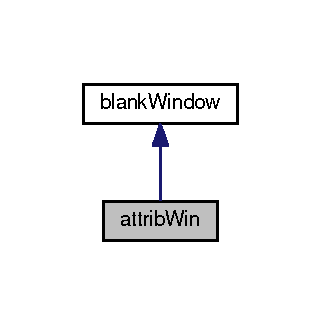
\includegraphics[width=154pt]{classgui_1_1window2_1_1attribWin__coll__graph}
\end{center}
\end{figure}
\subsection*{Public Member Functions}
\begin{DoxyCompactItemize}
\item 
\hypertarget{classgui_1_1window2_1_1attribWin_a615f3073891733337c33f599f89ec7ef}{def \hyperlink{classgui_1_1window2_1_1attribWin_a615f3073891733337c33f599f89ec7ef}{notdoneyet}}\label{classgui_1_1window2_1_1attribWin_a615f3073891733337c33f599f89ec7ef}

\begin{DoxyCompactList}\small\item\em Most important dummy method! \end{DoxyCompactList}\end{DoxyCompactItemize}


\subsection{Detailed Description}
This generates a window where attributes can be added to chosen elements of structure. 


\begin{DoxyParams}{Parameters}
{\em lang} & this holds the chosen display language. \\
\hline
{\em struc} & this holds the elements of structure in a dictionary \\
\hline
{\em filename} & name and path of the X\-M\-L file where the structure were read from. \\
\hline
{\em storepath} & path of the default storage location. \\
\hline
\end{DoxyParams}


The documentation for this class was generated from the following file\-:\begin{DoxyCompactItemize}
\item 
\hyperlink{window2_8py}{window2.\-py}\end{DoxyCompactItemize}

\hypertarget{classgui_1_1winhelper_1_1AutoScrollbar}{\section{Auto\-Scrollbar Class Reference}
\label{classgui_1_1winhelper_1_1AutoScrollbar}\index{Auto\-Scrollbar@{Auto\-Scrollbar}}
}


A scrollbar that hides itself if it's not needed.  




Inherits Scrollbar.

\subsection*{Public Member Functions}
\begin{DoxyCompactItemize}
\item 
\hypertarget{classgui_1_1winhelper_1_1AutoScrollbar_a494d5f53d3838090fc7841e90067e546}{def \hyperlink{classgui_1_1winhelper_1_1AutoScrollbar_a494d5f53d3838090fc7841e90067e546}{pack}}\label{classgui_1_1winhelper_1_1AutoScrollbar_a494d5f53d3838090fc7841e90067e546}

\begin{DoxyCompactList}\small\item\em Error handling method\-: This cannot be used with pack. \end{DoxyCompactList}\item 
\hypertarget{classgui_1_1winhelper_1_1AutoScrollbar_af53c142c14b9325d4c0ce56e8b230701}{def \hyperlink{classgui_1_1winhelper_1_1AutoScrollbar_af53c142c14b9325d4c0ce56e8b230701}{place}}\label{classgui_1_1winhelper_1_1AutoScrollbar_af53c142c14b9325d4c0ce56e8b230701}

\begin{DoxyCompactList}\small\item\em Error handling method\-: This cannot be used with place. \end{DoxyCompactList}\item 
\hypertarget{classgui_1_1winhelper_1_1AutoScrollbar_a621bd5e22d03cc48dbb784427b1c0fd8}{def \hyperlink{classgui_1_1winhelper_1_1AutoScrollbar_a621bd5e22d03cc48dbb784427b1c0fd8}{set}}\label{classgui_1_1winhelper_1_1AutoScrollbar_a621bd5e22d03cc48dbb784427b1c0fd8}

\begin{DoxyCompactList}\small\item\em sets or hides the scrollbar \end{DoxyCompactList}\end{DoxyCompactItemize}


\subsection{Detailed Description}
A scrollbar that hides itself if it's not needed. 

It only works if the grid geometry manager is used. 

The documentation for this class was generated from the following file\-:\begin{DoxyCompactItemize}
\item 
\hyperlink{winhelper_8py}{winhelper.\-py}\end{DoxyCompactItemize}

\input{classgui_1_1window_1_1blankWindow}
\hypertarget{classgui_1_1window2_1_1blankWindow}{\section{blank\-Window Class Reference}
\label{classgui_1_1window2_1_1blankWindow}\index{blank\-Window@{blank\-Window}}
}


A simple window class with a not filled menu bar.  




Inheritance diagram for blank\-Window\-:\nopagebreak
\begin{figure}[H]
\begin{center}
\leavevmode
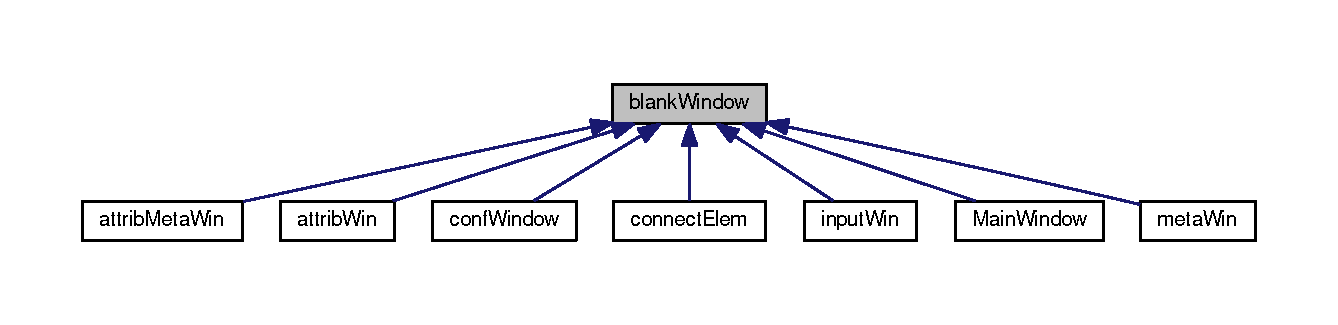
\includegraphics[width=350pt]{classgui_1_1window2_1_1blankWindow__inherit__graph}
\end{center}
\end{figure}
\subsection*{Public Member Functions}
\begin{DoxyCompactItemize}
\item 
\hypertarget{classgui_1_1window2_1_1blankWindow_a615f3073891733337c33f599f89ec7ef}{def \hyperlink{classgui_1_1window2_1_1blankWindow_a615f3073891733337c33f599f89ec7ef}{notdoneyet}}\label{classgui_1_1window2_1_1blankWindow_a615f3073891733337c33f599f89ec7ef}

\begin{DoxyCompactList}\small\item\em a simple dummy method for not yet implemented methods \end{DoxyCompactList}\end{DoxyCompactItemize}


\subsection{Detailed Description}
A simple window class with a not filled menu bar. 


\begin{DoxyParams}{Parameters}
{\em lang} & chosen language for the menu. \\
\hline
\end{DoxyParams}


The documentation for this class was generated from the following file\-:\begin{DoxyCompactItemize}
\item 
\hyperlink{window2_8py}{window2.\-py}\end{DoxyCompactItemize}

\input{classrpgtoolbox_1_1confbox_1_1chkCfg}
\input{classrpgToolDefinitions_1_1toolbox_1_1confbox_1_1chkCfg}
\hypertarget{classgui_1_1window2_1_1confWindow}{\section{conf\-Window Class Reference}
\label{classgui_1_1window2_1_1confWindow}\index{conf\-Window@{conf\-Window}}
}


This class builds a window for selecting and saving options of A\-Da\-Man\-T.  




Inheritance diagram for conf\-Window\-:\nopagebreak
\begin{figure}[H]
\begin{center}
\leavevmode
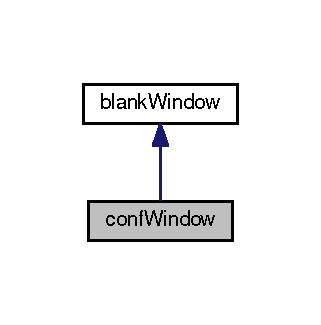
\includegraphics[width=154pt]{classgui_1_1window2_1_1confWindow__inherit__graph}
\end{center}
\end{figure}


Collaboration diagram for conf\-Window\-:\nopagebreak
\begin{figure}[H]
\begin{center}
\leavevmode
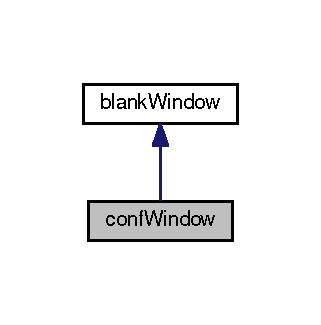
\includegraphics[width=154pt]{classgui_1_1window2_1_1confWindow__coll__graph}
\end{center}
\end{figure}
\subsection*{Public Member Functions}
\begin{DoxyCompactItemize}
\item 
\hypertarget{classgui_1_1window2_1_1confWindow_a2d2bfbe7abc45a786220f7555e52b01c}{def \hyperlink{classgui_1_1window2_1_1confWindow_a2d2bfbe7abc45a786220f7555e52b01c}{chosen\-Lang}}\label{classgui_1_1window2_1_1confWindow_a2d2bfbe7abc45a786220f7555e52b01c}

\begin{DoxyCompactList}\small\item\em A public method which return the string value of the chosen language. \end{DoxyCompactList}\end{DoxyCompactItemize}


\subsection{Detailed Description}
This class builds a window for selecting and saving options of A\-Da\-Man\-T. 

For now it is just chosing the language for menus and dialogues. 
\begin{DoxyParams}{Parameters}
{\em lang} & Laguage which shall be used in messages and menus. \\
\hline
\end{DoxyParams}


The documentation for this class was generated from the following file\-:\begin{DoxyCompactItemize}
\item 
\hyperlink{window2_8py}{window2.\-py}\end{DoxyCompactItemize}

\input{classgui_1_1window_1_1confWindow}
\hypertarget{classgui_1_1window2_1_1connectElem}{\section{connect\-Elem Class Reference}
\label{classgui_1_1window2_1_1connectElem}\index{connect\-Elem@{connect\-Elem}}
}


This creates a window to connect elements of structure logically.  




Inheritance diagram for connect\-Elem\-:\nopagebreak
\begin{figure}[H]
\begin{center}
\leavevmode
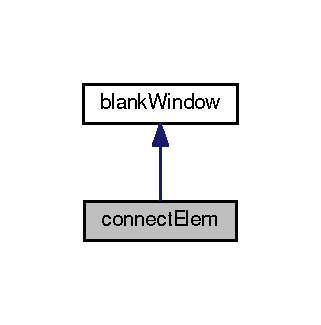
\includegraphics[width=154pt]{classgui_1_1window2_1_1connectElem__inherit__graph}
\end{center}
\end{figure}


Collaboration diagram for connect\-Elem\-:\nopagebreak
\begin{figure}[H]
\begin{center}
\leavevmode
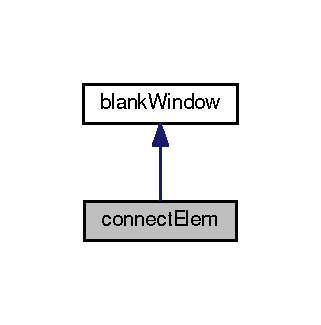
\includegraphics[width=154pt]{classgui_1_1window2_1_1connectElem__coll__graph}
\end{center}
\end{figure}
\subsection*{Public Member Functions}
\begin{DoxyCompactItemize}
\item 
\hypertarget{classgui_1_1window2_1_1connectElem_a615f3073891733337c33f599f89ec7ef}{def \hyperlink{classgui_1_1window2_1_1connectElem_a615f3073891733337c33f599f89ec7ef}{notdoneyet}}\label{classgui_1_1window2_1_1connectElem_a615f3073891733337c33f599f89ec7ef}

\begin{DoxyCompactList}\small\item\em Most important dummy method! \end{DoxyCompactList}\end{DoxyCompactItemize}


\subsection{Detailed Description}
This creates a window to connect elements of structure logically. 


\begin{DoxyParams}{Parameters}
{\em lang} & holds the chosen diplay language \\
\hline
{\em struc} & holds a ditionary with the funtional structure \\
\hline
{\em filename} & contains the filename and path where the structure may be read from \\
\hline
{\em storepath} & holds the default storage location for the X\-M\-L files. \\
\hline
\end{DoxyParams}


The documentation for this class was generated from the following file\-:\begin{DoxyCompactItemize}
\item 
\hyperlink{window2_8py}{window2.\-py}\end{DoxyCompactItemize}

\hypertarget{classgui_1_1window2_1_1drawTree}{\section{draw\-Tree Class Reference}
\label{classgui_1_1window2_1_1drawTree}\index{draw\-Tree@{draw\-Tree}}
}


This class creates an object to draw a graph of a tree structure (in a dictionary).  




Inherits object.

\subsection*{Public Member Functions}
\begin{DoxyCompactItemize}
\item 
\hypertarget{classgui_1_1window2_1_1drawTree_a615f3073891733337c33f599f89ec7ef}{def \hyperlink{classgui_1_1window2_1_1drawTree_a615f3073891733337c33f599f89ec7ef}{notdoneyet}}\label{classgui_1_1window2_1_1drawTree_a615f3073891733337c33f599f89ec7ef}

\begin{DoxyCompactList}\small\item\em a simple dummy method for not yet implemented methods \end{DoxyCompactList}\end{DoxyCompactItemize}


\subsection{Detailed Description}
This class creates an object to draw a graph of a tree structure (in a dictionary). 


\begin{DoxyParams}{Parameters}
{\em lang} & contains the used language. \\
\hline
{\em struc} & contains the structure of the tree \\
\hline
{\em parent} & key for the parent index list in the dictionary \\
\hline
{\em child} & key for the child index list in the dictionary \\
\hline
\end{DoxyParams}


The documentation for this class was generated from the following file\-:\begin{DoxyCompactItemize}
\item 
\hyperlink{window2_8py}{window2.\-py}\end{DoxyCompactItemize}

\input{classrpgToolDefinitions_1_1toolbox_1_1xmltools_1_1handleXML}
\hypertarget{classgui_1_1winhelper_1_1InfoCanvas}{\section{Info\-Canvas Class Reference}
\label{classgui_1_1winhelper_1_1InfoCanvas}\index{Info\-Canvas@{Info\-Canvas}}
}


A Canvas-\/widget that holds a scrollable Message-\/widget.  




Inherits object.

\subsection*{Public Member Functions}
\begin{DoxyCompactItemize}
\item 
\hypertarget{classgui_1_1winhelper_1_1InfoCanvas_a494d5f53d3838090fc7841e90067e546}{def \hyperlink{classgui_1_1winhelper_1_1InfoCanvas_a494d5f53d3838090fc7841e90067e546}{pack}}\label{classgui_1_1winhelper_1_1InfoCanvas_a494d5f53d3838090fc7841e90067e546}

\begin{DoxyCompactList}\small\item\em Error handling method\-: This cannot be used with pack. \end{DoxyCompactList}\item 
\hypertarget{classgui_1_1winhelper_1_1InfoCanvas_af53c142c14b9325d4c0ce56e8b230701}{def \hyperlink{classgui_1_1winhelper_1_1InfoCanvas_af53c142c14b9325d4c0ce56e8b230701}{place}}\label{classgui_1_1winhelper_1_1InfoCanvas_af53c142c14b9325d4c0ce56e8b230701}

\begin{DoxyCompactList}\small\item\em Error handling method\-: This cannot be used with place. \end{DoxyCompactList}\end{DoxyCompactItemize}


\subsection{Detailed Description}
A Canvas-\/widget that holds a scrollable Message-\/widget. 

This widget can only be used by the grid() Geometry Manager.


\begin{DoxyParams}{Parameters}
{\em master} & master Tk()-\/object \\
\hline
{\em text} & text string that shall be displayed \\
\hline
{\em width} & width of the canvas in pixel \\
\hline
{\em row} & row index where to put this widget in the window structure \\
\hline
{\em column} & column index where to put this widget in the window structure \\
\hline
\end{DoxyParams}


The documentation for this class was generated from the following file\-:\begin{DoxyCompactItemize}
\item 
\hyperlink{winhelper_8py}{winhelper.\-py}\end{DoxyCompactItemize}

\input{classgui_1_1window_1_1inputWin}
\hypertarget{classgui_1_1window2_1_1inputWin}{\section{input\-Win Class Reference}
\label{classgui_1_1window2_1_1inputWin}\index{input\-Win@{input\-Win}}
}


Objects of this class type are windows for input the wanted data structure.  




Inheritance diagram for input\-Win\-:\nopagebreak
\begin{figure}[H]
\begin{center}
\leavevmode
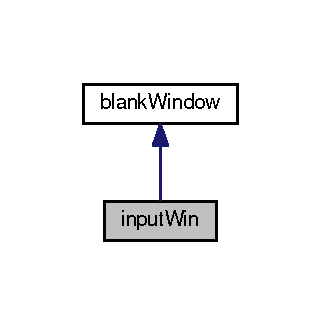
\includegraphics[width=154pt]{classgui_1_1window2_1_1inputWin__inherit__graph}
\end{center}
\end{figure}


Collaboration diagram for input\-Win\-:\nopagebreak
\begin{figure}[H]
\begin{center}
\leavevmode
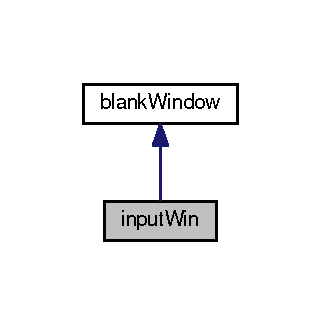
\includegraphics[width=154pt]{classgui_1_1window2_1_1inputWin__coll__graph}
\end{center}
\end{figure}
\subsection*{Public Member Functions}
\begin{DoxyCompactItemize}
\item 
def \hyperlink{classgui_1_1window2_1_1inputWin_a0a4ec80f6a730ee05d9650bad587d74f}{create\-Win\-Struc}
\begin{DoxyCompactList}\small\item\em This method creates the window structure with list and message boxes. \end{DoxyCompactList}\item 
\hypertarget{classgui_1_1window2_1_1inputWin_a615f3073891733337c33f599f89ec7ef}{def \hyperlink{classgui_1_1window2_1_1inputWin_a615f3073891733337c33f599f89ec7ef}{notdoneyet}}\label{classgui_1_1window2_1_1inputWin_a615f3073891733337c33f599f89ec7ef}

\begin{DoxyCompactList}\small\item\em Most important dummy method! \end{DoxyCompactList}\end{DoxyCompactItemize}


\subsection{Detailed Description}
Objects of this class type are windows for input the wanted data structure. 

A X\-M\-L structure will be build of the input. 
\begin{DoxyParams}{Parameters}
{\em lang} & This parameter holds the language chosen for the menus and messages. Default value is 'en'. \\
\hline
{\em xmlcontent} & a dictionary holding the X\-M\-L structure/tags \\
\hline
{\em filename} & this holds the filename of a read X\-M\-L file holding the functional structure. \\
\hline
{\em storepath} & the path where the X\-M\-L files shall be stored in. \\
\hline
\end{DoxyParams}


\subsection{Member Function Documentation}
\hypertarget{classgui_1_1window2_1_1inputWin_a0a4ec80f6a730ee05d9650bad587d74f}{\index{gui\-::window2\-::input\-Win@{gui\-::window2\-::input\-Win}!create\-Win\-Struc@{create\-Win\-Struc}}
\index{create\-Win\-Struc@{create\-Win\-Struc}!gui::window2::inputWin@{gui\-::window2\-::input\-Win}}
\subsubsection[{create\-Win\-Struc}]{\setlength{\rightskip}{0pt plus 5cm}def create\-Win\-Struc (
\begin{DoxyParamCaption}
\item[{}]{self}
\end{DoxyParamCaption}
)}}\label{classgui_1_1window2_1_1inputWin_a0a4ec80f6a730ee05d9650bad587d74f}


This method creates the window structure with list and message boxes. 

The created window is for reading, generating and editing of elements of the functional structure. 

Here is the call graph for this function\-:\nopagebreak
\begin{figure}[H]
\begin{center}
\leavevmode
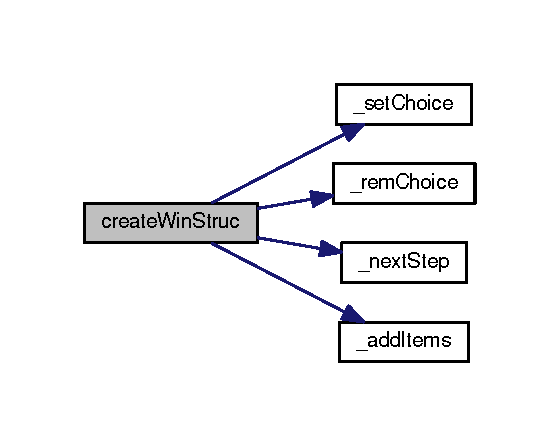
\includegraphics[width=268pt]{classgui_1_1window2_1_1inputWin_a0a4ec80f6a730ee05d9650bad587d74f_cgraph}
\end{center}
\end{figure}




The documentation for this class was generated from the following file\-:\begin{DoxyCompactItemize}
\item 
\hyperlink{window2_8py}{window2.\-py}\end{DoxyCompactItemize}

\input{classrpgToolDefinitions_1_1MERSTables_1_1Magic}
\input{classgui_1_1window_1_1MainWindow}
\input{classcalc__ep_1_1MainWindow}
\hypertarget{classgui_1_1window2_1_1MainWindow}{\section{Main\-Window Class Reference}
\label{classgui_1_1window2_1_1MainWindow}\index{Main\-Window@{Main\-Window}}
}


This is the class for the main window object.  




Inheritance diagram for Main\-Window\-:\nopagebreak
\begin{figure}[H]
\begin{center}
\leavevmode
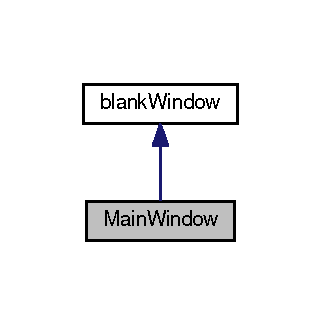
\includegraphics[width=154pt]{classgui_1_1window2_1_1MainWindow__inherit__graph}
\end{center}
\end{figure}


Collaboration diagram for Main\-Window\-:\nopagebreak
\begin{figure}[H]
\begin{center}
\leavevmode
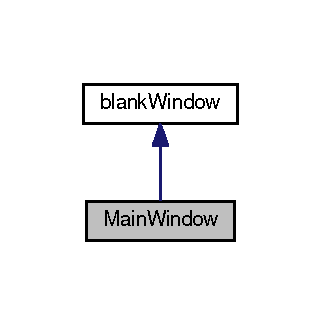
\includegraphics[width=154pt]{classgui_1_1window2_1_1MainWindow__coll__graph}
\end{center}
\end{figure}
\subsection*{Public Member Functions}
\begin{DoxyCompactItemize}
\item 
\hypertarget{classgui_1_1window2_1_1MainWindow_ad4f4bbba4c4a628d0a35195b093d6049}{def \hyperlink{classgui_1_1window2_1_1MainWindow_ad4f4bbba4c4a628d0a35195b093d6049}{help\-About}}\label{classgui_1_1window2_1_1MainWindow_ad4f4bbba4c4a628d0a35195b093d6049}

\begin{DoxyCompactList}\small\item\em This method just opens a message window with the basic information about the A\-Da\-Man\-T X\-M\-L Generator (like version and copyright) \end{DoxyCompactList}\item 
def \hyperlink{classgui_1_1window2_1_1MainWindow_a784d15d1157ea5b181c63d73daa3fc5e}{help\-Handbook}
\begin{DoxyCompactList}\small\item\em This method will show the A\-Da\-Man\-T Handbook. \end{DoxyCompactList}\item 
\hypertarget{classgui_1_1window2_1_1MainWindow_a615f3073891733337c33f599f89ec7ef}{def \hyperlink{classgui_1_1window2_1_1MainWindow_a615f3073891733337c33f599f89ec7ef}{notdoneyet}}\label{classgui_1_1window2_1_1MainWindow_a615f3073891733337c33f599f89ec7ef}

\begin{DoxyCompactList}\small\item\em An I\-M\-P\-O\-R\-T\-A\-N\-T dummy for methods which are not implemented yet ;-\/) \end{DoxyCompactList}\item 
\hypertarget{classgui_1_1window2_1_1MainWindow_a2cc0c3d64b049aac95bc9fdbb9673050}{def \hyperlink{classgui_1_1window2_1_1MainWindow_a2cc0c3d64b049aac95bc9fdbb9673050}{opt\-Win}}\label{classgui_1_1window2_1_1MainWindow_a2cc0c3d64b049aac95bc9fdbb9673050}

\begin{DoxyCompactList}\small\item\em Opens an option window and closes the main window. \end{DoxyCompactList}\end{DoxyCompactItemize}


\subsection{Detailed Description}
This is the class for the main window object. 


\begin{DoxyParams}{Parameters}
{\em lang} & The chosen language for window's and button's texts. At the moment, only English (en, default value) and German (de) are supported. \\
\hline
\end{DoxyParams}


\subsection{Member Function Documentation}
\hypertarget{classgui_1_1window2_1_1MainWindow_a784d15d1157ea5b181c63d73daa3fc5e}{\index{gui\-::window2\-::\-Main\-Window@{gui\-::window2\-::\-Main\-Window}!help\-Handbook@{help\-Handbook}}
\index{help\-Handbook@{help\-Handbook}!gui::window2::MainWindow@{gui\-::window2\-::\-Main\-Window}}
\subsubsection[{help\-Handbook}]{\setlength{\rightskip}{0pt plus 5cm}def help\-Handbook (
\begin{DoxyParamCaption}
\item[{}]{self}
\end{DoxyParamCaption}
)}}\label{classgui_1_1window2_1_1MainWindow_a784d15d1157ea5b181c63d73daa3fc5e}


This method will show the A\-Da\-Man\-T Handbook. 

\begin{DoxyRefDesc}{Todo}
\item[\hyperlink{todo__todo000011}{Todo}]this needs to be implemented \end{DoxyRefDesc}


Here is the call graph for this function\-:
\nopagebreak
\begin{figure}[H]
\begin{center}
\leavevmode
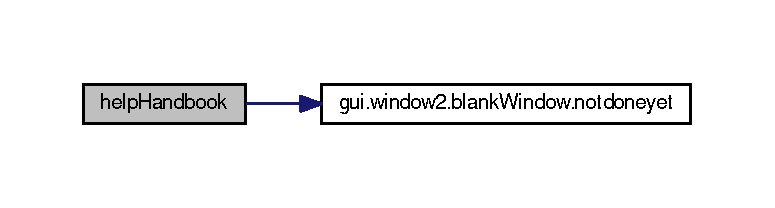
\includegraphics[height=550pt]{classgui_1_1window2_1_1MainWindow_a784d15d1157ea5b181c63d73daa3fc5e_cgraph}
\end{center}
\end{figure}




Here is the caller graph for this function\-:\nopagebreak
\begin{figure}[H]
\begin{center}
\leavevmode
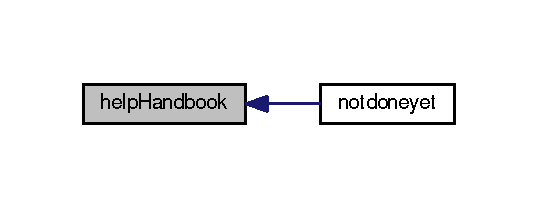
\includegraphics[width=258pt]{classgui_1_1window2_1_1MainWindow_a784d15d1157ea5b181c63d73daa3fc5e_icgraph}
\end{center}
\end{figure}




The documentation for this class was generated from the following file\-:\begin{DoxyCompactItemize}
\item 
\hyperlink{window2_8py}{window2.\-py}\end{DoxyCompactItemize}

\hypertarget{classgui_1_1window3_1_1MenuWin}{\section{Menu\-Win Class Reference}
\label{classgui_1_1window3_1_1MenuWin}\index{Menu\-Win@{Menu\-Win}}
}


Master class for all windows using menus.  




Inherits object.

\subsection*{Public Member Functions}
\begin{DoxyCompactItemize}
\item 
def \hyperlink{classgui_1_1window3_1_1MenuWin_ab66f1da42371ac6f08a9817adf59a38e}{add\-Help}
\begin{DoxyCompactList}\small\item\em This method adds a help menu to the menu bar. \end{DoxyCompactList}\item 
def \hyperlink{classgui_1_1window3_1_1MenuWin_a4b810e6adc7d147eaa8edb45dd5891ca}{context\-Help}
\begin{DoxyCompactList}\small\item\em This method opens a context help window where the user may get more detailed help information about the task he is doing. \end{DoxyCompactList}\item 
def \hyperlink{classgui_1_1window3_1_1MenuWin_a2e91f76cce6e9b7a03830202f45aecf0}{first\-Steps}
\begin{DoxyCompactList}\small\item\em This method opens a help window with the first steps howtos. \end{DoxyCompactList}\item 
\hypertarget{classgui_1_1window3_1_1MenuWin_ad4f4bbba4c4a628d0a35195b093d6049}{def \hyperlink{classgui_1_1window3_1_1MenuWin_ad4f4bbba4c4a628d0a35195b093d6049}{help\-About}}\label{classgui_1_1window3_1_1MenuWin_ad4f4bbba4c4a628d0a35195b093d6049}

\begin{DoxyCompactList}\small\item\em This method just opens a message window with the basic information about the A\-Da\-Man\-T X\-M\-L Generator (like version and copyright) \end{DoxyCompactList}\end{DoxyCompactItemize}


\subsection{Detailed Description}
Master class for all windows using menus. 

It just contains a basic window layout with a menu bar. There is a method for a help menu, but it is not linked to the menu bar yet. 
\begin{DoxyParams}{Parameters}
{\em lang} & This parameter holds the language that should be used for the G\-U\-I's texts. At the moment, German (de) and English (en) are supported. Default language is English. \\
\hline
\end{DoxyParams}


\subsection{Member Function Documentation}
\hypertarget{classgui_1_1window3_1_1MenuWin_ab66f1da42371ac6f08a9817adf59a38e}{\index{gui\-::window3\-::\-Menu\-Win@{gui\-::window3\-::\-Menu\-Win}!add\-Help@{add\-Help}}
\index{add\-Help@{add\-Help}!gui::window3::MenuWin@{gui\-::window3\-::\-Menu\-Win}}
\subsubsection[{add\-Help}]{\setlength{\rightskip}{0pt plus 5cm}def add\-Help (
\begin{DoxyParamCaption}
\item[{}]{self, }
\item[{}]{context = {\ttfamily 'hlp\-\_\-about'}}
\end{DoxyParamCaption}
)}}\label{classgui_1_1window3_1_1MenuWin_ab66f1da42371ac6f08a9817adf59a38e}


This method adds a help menu to the menu bar. 


\begin{DoxyParams}{Parameters}
{\em context} & defines the context of the needed help menu\-: e.\-g., an {\itshape about} {\itshape information} (which is the default)\\
\hline
\end{DoxyParams}
\begin{DoxyRefDesc}{Todo}
\item[\hyperlink{todo__todo000024}{Todo}]\-: add additional help contexts -\/ maybe even a real {\itshape context} {\itshape help} \end{DoxyRefDesc}


Here is the call graph for this function\-:\nopagebreak
\begin{figure}[H]
\begin{center}
\leavevmode
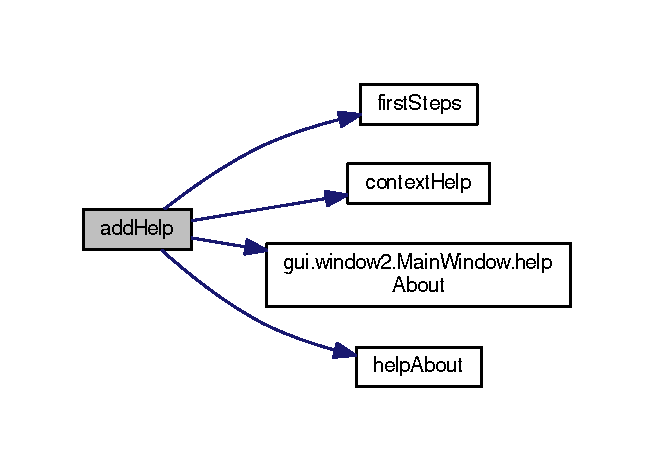
\includegraphics[width=322pt]{classgui_1_1window3_1_1MenuWin_ab66f1da42371ac6f08a9817adf59a38e_cgraph}
\end{center}
\end{figure}


\hypertarget{classgui_1_1window3_1_1MenuWin_a4b810e6adc7d147eaa8edb45dd5891ca}{\index{gui\-::window3\-::\-Menu\-Win@{gui\-::window3\-::\-Menu\-Win}!context\-Help@{context\-Help}}
\index{context\-Help@{context\-Help}!gui::window3::MenuWin@{gui\-::window3\-::\-Menu\-Win}}
\subsubsection[{context\-Help}]{\setlength{\rightskip}{0pt plus 5cm}def context\-Help (
\begin{DoxyParamCaption}
\item[{}]{self}
\end{DoxyParamCaption}
)}}\label{classgui_1_1window3_1_1MenuWin_a4b810e6adc7d147eaa8edb45dd5891ca}


This method opens a context help window where the user may get more detailed help information about the task he is doing. 

\begin{DoxyRefDesc}{Todo}
\item[\hyperlink{todo__todo000026}{Todo}]\-: Implement a context help method \end{DoxyRefDesc}


Here is the caller graph for this function\-:\nopagebreak
\begin{figure}[H]
\begin{center}
\leavevmode
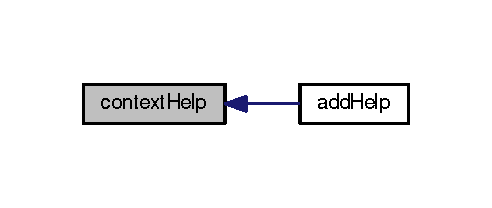
\includegraphics[width=236pt]{classgui_1_1window3_1_1MenuWin_a4b810e6adc7d147eaa8edb45dd5891ca_icgraph}
\end{center}
\end{figure}


\hypertarget{classgui_1_1window3_1_1MenuWin_a2e91f76cce6e9b7a03830202f45aecf0}{\index{gui\-::window3\-::\-Menu\-Win@{gui\-::window3\-::\-Menu\-Win}!first\-Steps@{first\-Steps}}
\index{first\-Steps@{first\-Steps}!gui::window3::MenuWin@{gui\-::window3\-::\-Menu\-Win}}
\subsubsection[{first\-Steps}]{\setlength{\rightskip}{0pt plus 5cm}def first\-Steps (
\begin{DoxyParamCaption}
\item[{}]{self}
\end{DoxyParamCaption}
)}}\label{classgui_1_1window3_1_1MenuWin_a2e91f76cce6e9b7a03830202f45aecf0}


This method opens a help window with the first steps howtos. 

\begin{DoxyRefDesc}{Todo}
\item[\hyperlink{todo__todo000025}{Todo}]\-: implement this help method 

\-: write the first step howtos... \end{DoxyRefDesc}


Here is the caller graph for this function\-:\nopagebreak
\begin{figure}[H]
\begin{center}
\leavevmode
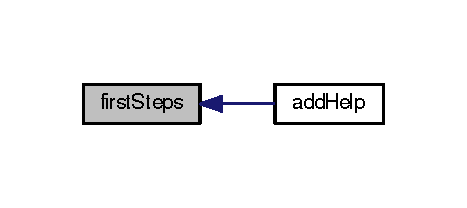
\includegraphics[width=224pt]{classgui_1_1window3_1_1MenuWin_a2e91f76cce6e9b7a03830202f45aecf0_icgraph}
\end{center}
\end{figure}




The documentation for this class was generated from the following file\-:\begin{DoxyCompactItemize}
\item 
\hyperlink{window3_8py}{window3.\-py}\end{DoxyCompactItemize}

\input{classgui_1_1window_1_1messageWindow}
\hypertarget{classgui_1_1window2_1_1messageWindow}{\section{message\-Window \-Class \-Reference}
\label{classgui_1_1window2_1_1messageWindow}\index{message\-Window@{message\-Window}}
}


\-A class to build a message window containing version, author and email on default.  


\subsection*{\-Public \-Member \-Functions}
\begin{DoxyCompactItemize}
\item 
def \hyperlink{classgui_1_1window2_1_1messageWindow_a96cedc16e980eef3f1fb0412418201c6}{showinfo}
\begin{DoxyCompactList}\small\item\em \-This method adds and displays content to the message window. \end{DoxyCompactList}\end{DoxyCompactItemize}


\subsection{\-Detailed \-Description}
\-A class to build a message window containing version, author and email on default. 


\begin{DoxyParams}{\-Parameters}
{\em lang} & contains the chosen display language. \\
\hline
\end{DoxyParams}


\subsection{\-Member \-Function \-Documentation}
\hypertarget{classgui_1_1window2_1_1messageWindow_a96cedc16e980eef3f1fb0412418201c6}{\index{gui\-::window2\-::message\-Window@{gui\-::window2\-::message\-Window}!showinfo@{showinfo}}
\index{showinfo@{showinfo}!gui::window2::messageWindow@{gui\-::window2\-::message\-Window}}
\subsubsection[{showinfo}]{\setlength{\rightskip}{0pt plus 5cm}def {\bf showinfo} (
\begin{DoxyParamCaption}
\item[{}]{self, }
\item[{}]{message = {\ttfamily ''}, }
\item[{}]{title = {\ttfamily '\-Info'}}
\end{DoxyParamCaption}
)}}\label{classgui_1_1window2_1_1messageWindow_a96cedc16e980eef3f1fb0412418201c6}


\-This method adds and displays content to the message window. 


\begin{DoxyParams}{\-Parameters}
{\em message} & contains a message to be displayed in the message window. \-It may be an array, a string or a number (integer/float). \\
\hline
{\em title} & sets the title of the message window. \-The default is '\-Info'. \\
\hline
\end{DoxyParams}


\-References message\-Window.\-lang, message\-Window.\-title, and message\-Window.\-window.



\-The documentation for this class was generated from the following file\-:\begin{DoxyCompactItemize}
\item 
window2.\-py\end{DoxyCompactItemize}

\hypertarget{classgui_1_1window3_1_1messageWindow}{\section{message\-Window Class Reference}
\label{classgui_1_1window3_1_1messageWindow}\index{message\-Window@{message\-Window}}
}


A class to build a message window containing version, author and email on default.  




Inherits object.

\subsection*{Public Member Functions}
\begin{DoxyCompactItemize}
\item 
def \hyperlink{classgui_1_1window3_1_1messageWindow_a96cedc16e980eef3f1fb0412418201c6}{showinfo}
\begin{DoxyCompactList}\small\item\em This method adds content to the message window. \end{DoxyCompactList}\end{DoxyCompactItemize}


\subsection{Detailed Description}
A class to build a message window containing version, author and email on default. 

\subsection{Member Function Documentation}
\hypertarget{classgui_1_1window3_1_1messageWindow_a96cedc16e980eef3f1fb0412418201c6}{\index{gui\-::window3\-::message\-Window@{gui\-::window3\-::message\-Window}!showinfo@{showinfo}}
\index{showinfo@{showinfo}!gui::window3::messageWindow@{gui\-::window3\-::message\-Window}}
\subsubsection[{showinfo}]{\setlength{\rightskip}{0pt plus 5cm}def showinfo (
\begin{DoxyParamCaption}
\item[{}]{self, }
\item[{}]{message = {\ttfamily ''}, }
\item[{}]{title = {\ttfamily 'Info'}}
\end{DoxyParamCaption}
)}}\label{classgui_1_1window3_1_1messageWindow_a96cedc16e980eef3f1fb0412418201c6}


This method adds content to the message window. 


\begin{DoxyParams}{Parameters}
{\em message} & contains a message to be displayed in the message window. It may be an array, a string or a number (integer/float). \\
\hline
{\em title} & sets the title of the message window. The default is 'Info'. \\
\hline
\end{DoxyParams}


The documentation for this class was generated from the following file\-:\begin{DoxyCompactItemize}
\item 
\hyperlink{window3_8py}{window3.\-py}\end{DoxyCompactItemize}

\input{classgui_1_1window_1_1metaWin}
\hypertarget{classgui_1_1window2_1_1metaWin}{\section{meta\-Win Class Reference}
\label{classgui_1_1window2_1_1metaWin}\index{meta\-Win@{meta\-Win}}
}


Creates a window for generating meta data fields.  




Inheritance diagram for meta\-Win\-:\nopagebreak
\begin{figure}[H]
\begin{center}
\leavevmode
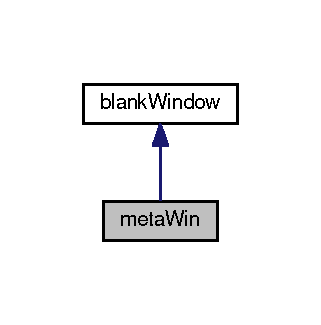
\includegraphics[width=154pt]{classgui_1_1window2_1_1metaWin__inherit__graph}
\end{center}
\end{figure}


Collaboration diagram for meta\-Win\-:\nopagebreak
\begin{figure}[H]
\begin{center}
\leavevmode
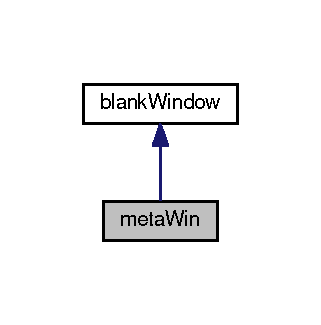
\includegraphics[width=154pt]{classgui_1_1window2_1_1metaWin__coll__graph}
\end{center}
\end{figure}
\subsection*{Public Member Functions}
\begin{DoxyCompactItemize}
\item 
\hypertarget{classgui_1_1window2_1_1metaWin_a615f3073891733337c33f599f89ec7ef}{def \hyperlink{classgui_1_1window2_1_1metaWin_a615f3073891733337c33f599f89ec7ef}{notdoneyet}}\label{classgui_1_1window2_1_1metaWin_a615f3073891733337c33f599f89ec7ef}

\begin{DoxyCompactList}\small\item\em Most important dummy method! \end{DoxyCompactList}\end{DoxyCompactItemize}


\subsection{Detailed Description}
Creates a window for generating meta data fields. 


\begin{DoxyParams}{Parameters}
{\em lang} & this holds the chosen display language. \\
\hline
{\em struc} & this holds the elements of structure in a dictionary \\
\hline
{\em struc} & this holds the elements of meta data in a dictionary \\
\hline
{\em fn\-\_\-struc} & path and name of the X\-M\-L file where the structure were read from. \\
\hline
{\em fn\-\_\-meta} & path and name of the X\-M\-L file where the meta data will be saved in. \\
\hline
{\em storepath} & path of the default storage location of the X\-M\-L files. \\
\hline
\end{DoxyParams}


The documentation for this class was generated from the following file\-:\begin{DoxyCompactItemize}
\item 
\hyperlink{window2_8py}{window2.\-py}\end{DoxyCompactItemize}

\input{classrpgToolDefinitions_1_1RMTables_1_1MyClass}
\chapter{File Documentation}
\hypertarget{Backpack_8py}{\section{Backpack.\-py File Reference}
\label{Backpack_8py}\index{Backpack.\-py@{Backpack.\-py}}
}


This is a simple tool to keep track of a character's backpack.  




\subsection{Detailed Description}
This is a simple tool to keep track of a character's backpack. With this tool you are able to keep track of all the items and the money a pen \& paper R\-P\-G character is carrying. To make it work as an \char`\"{}\-Online Shop\char`\"{} you need to set up a My\-S\-Q\-L data base.

\begin{DoxyDate}{Date}
(C) 2015 
\end{DoxyDate}
\begin{DoxyAuthor}{Author}
Marcus Schwamberger  \href{mailto:marcus@lederzeug.de}{\tt marcus@lederzeug.\-de}
\end{DoxyAuthor}
\begin{DoxyRefDesc}{Todo}
\item[\hyperlink{todo__todo000001}{Todo}]Modul\-: reading and interpreting mysql configuration 

Modul\-: create intial mysql db 

Modul\-: insert, update and read data from db 

Modul\-: saves extracted data as P\-D\-F \end{DoxyRefDesc}

\input{calc__ep_8py}
\input{rpgToolDefinitions_2epcalcdefs_8py}
\input{helptools_8py}
\input{itemshop_8py}
\input{MERSTables_8py}
\input{rpgtools_8py}
\input{window_8py}
\hypertarget{window2_8py}{\section{window2.\-py File Reference}
\label{window2_8py}\index{window2.\-py@{window2.\-py}}
}


All classes and functions for Tk used for Python 2.\-6+.  


\subsection*{Data Structures}
\begin{DoxyCompactItemize}
\item 
class \hyperlink{classgui_1_1window2_1_1attribMetaWin}{attrib\-Meta\-Win}
\begin{DoxyCompactList}\small\item\em This opens a window for setting the attributes of meta data fields. \end{DoxyCompactList}\item 
class \hyperlink{classgui_1_1window2_1_1attribWin}{attrib\-Win}
\begin{DoxyCompactList}\small\item\em This generates a window where attributes can be added to chosen elements of structure. \end{DoxyCompactList}\item 
class \hyperlink{classgui_1_1window2_1_1blankWindow}{blank\-Window}
\begin{DoxyCompactList}\small\item\em A simple window class with a not filled menu bar. \end{DoxyCompactList}\item 
class \hyperlink{classgui_1_1window2_1_1confWindow}{conf\-Window}
\begin{DoxyCompactList}\small\item\em This class builds a window for selecting and saving options of A\-Da\-Man\-T. \end{DoxyCompactList}\item 
class \hyperlink{classgui_1_1window2_1_1connectElem}{connect\-Elem}
\begin{DoxyCompactList}\small\item\em This creates a window to connect elements of structure logically. \end{DoxyCompactList}\item 
class \hyperlink{classgui_1_1window2_1_1drawTree}{draw\-Tree}
\begin{DoxyCompactList}\small\item\em This class creates an object to draw a graph of a tree structure (in a dictionary). \end{DoxyCompactList}\item 
class \hyperlink{classgui_1_1window2_1_1inputWin}{input\-Win}
\begin{DoxyCompactList}\small\item\em Objects of this class type are windows for input the wanted data structure. \end{DoxyCompactList}\item 
class \hyperlink{classgui_1_1window2_1_1MainWindow}{Main\-Window}
\begin{DoxyCompactList}\small\item\em This is the class for the main window object. \end{DoxyCompactList}\item 
class \hyperlink{classgui_1_1window2_1_1messageWindow}{message\-Window}
\begin{DoxyCompactList}\small\item\em A class to build a message window containing version, author and email on default. \end{DoxyCompactList}\item 
class \hyperlink{classgui_1_1window2_1_1metaWin}{meta\-Win}
\begin{DoxyCompactList}\small\item\em Creates a window for generating meta data fields. \end{DoxyCompactList}\end{DoxyCompactItemize}


\subsection{Detailed Description}
All classes and functions for Tk used for Python 2.\-6+. This module contains all needed classes/functions to build up a G\-U\-I with Tk and Python 2.\-6+

\begin{DoxyAuthor}{Author}
Marcus Schwamberger  \href{mailto:Marcus@lederzeug.de}{\tt Marcus@lederzeug.\-de} 
\end{DoxyAuthor}
\begin{DoxyDate}{Date}
(c) 2015 
\end{DoxyDate}
\begin{DoxyVersion}{Version}
1.\-0a 
\end{DoxyVersion}

\hypertarget{window3_8py}{\section{window3.\-py File Reference}
\label{window3_8py}\index{window3.\-py@{window3.\-py}}
}


All classes and functions for Tk used for Python 3.\-x.  


\subsection*{Data Structures}
\begin{DoxyCompactItemize}
\item 
class \hyperlink{classgui_1_1window3_1_1MenuWin}{Menu\-Win}
\begin{DoxyCompactList}\small\item\em Master class for all windows using menus. \end{DoxyCompactList}\item 
class \hyperlink{classgui_1_1window3_1_1messageWindow}{message\-Window}
\begin{DoxyCompactList}\small\item\em A class to build a message window containing version, author and email on default. \end{DoxyCompactList}\end{DoxyCompactItemize}


\subsection{Detailed Description}
All classes and functions for Tk used for Python 3.\-x. This module contains all needed classes/functions to build up a G\-U\-I with Tk and Python 3.\-x

\begin{DoxyAuthor}{Author}
Marcus Schwamberger  \href{mailto:marcus@lederzeug.de}{\tt marcus@lederzeug.\-de} 
\end{DoxyAuthor}
\begin{DoxyDate}{Date}
(c) 2012 
\end{DoxyDate}
\begin{DoxyVersion}{Version}
0.\-1 alpha 
\end{DoxyVersion}

\hypertarget{winhelper_8py}{\section{winhelper.\-py File Reference}
\label{winhelper_8py}\index{winhelper.\-py@{winhelper.\-py}}
}


collection of helper tools for building Tk() windows/apps  


\subsection*{Data Structures}
\begin{DoxyCompactItemize}
\item 
class \hyperlink{classgui_1_1winhelper_1_1AutoScrollbar}{Auto\-Scrollbar}
\begin{DoxyCompactList}\small\item\em A scrollbar that hides itself if it's not needed. \end{DoxyCompactList}\item 
class \hyperlink{classgui_1_1winhelper_1_1InfoCanvas}{Info\-Canvas}
\begin{DoxyCompactList}\small\item\em A Canvas-\/widget that holds a scrollable Message-\/widget. \end{DoxyCompactList}\end{DoxyCompactItemize}
\subsection*{Functions}
\begin{DoxyCompactItemize}
\item 
def {\bfseries build\-Win\-Check}
\begin{DoxyCompactList}\small\item\em This function is a little helper for building windows with check buttons. \end{DoxyCompactList}\item 
def {\bfseries build\-Win\-Radio}
\begin{DoxyCompactList}\small\item\em This function is a little helper to build with radio buttons. \end{DoxyCompactList}\end{DoxyCompactItemize}


\subsection{Detailed Description}
collection of helper tools for building Tk() windows/apps \begin{DoxyDate}{Date}
(C) 2012 
\end{DoxyDate}
\begin{DoxyAuthor}{Author}
Marcus Schwamberger  \href{mailto:marcus@lederzeug.de}{\tt marcus@lederzeug.\-de} 
\end{DoxyAuthor}
\begin{DoxyVersion}{Version}
0.\-5.\-4 alpha 
\end{DoxyVersion}

\hypertarget{xmlbox_8py}{\section{xmlbox.\-py File Reference}
\label{xmlbox_8py}\index{xmlbox.\-py@{xmlbox.\-py}}
}


This module contains needed X\-M\-L tools.  


\subsection*{Variables}
\begin{DoxyCompactItemize}
\item 
\hypertarget{namespacetoolbox_1_1xmlbox_a490de5e0ba80d41882b64a6bb1618ccb}{dictionary {\bfseries attrib\-\_\-metad}}\label{namespacetoolbox_1_1xmlbox_a490de5e0ba80d41882b64a6bb1618ccb}

\begin{DoxyCompactList}\small\item\em attrib\-\_\-metad Allowed attributes for metadata elements \end{DoxyCompactList}\item 
\hypertarget{namespacetoolbox_1_1xmlbox_a03c4bff8a46b0b0825d5a5043b608d1c}{dictionary {\bfseries attrib\-\_\-struc}}\label{namespacetoolbox_1_1xmlbox_a03c4bff8a46b0b0825d5a5043b608d1c}

\begin{DoxyCompactList}\small\item\em attrib\-\_\-struct Allowed attributes for functional elements of structure \end{DoxyCompactList}\item 
dictionary {\bfseries struct}
\begin{DoxyCompactList}\small\item\em struct holds the default data structure. \end{DoxyCompactList}\end{DoxyCompactItemize}


\subsection{Detailed Description}
This module contains needed X\-M\-L tools. \begin{DoxyDate}{Date}
(C) 2012 
\end{DoxyDate}
\begin{DoxyAuthor}{Author}
Marcus Schwamberger  \href{mailto:marcus@lederzeug.de}{\tt marcus@lederzeug.\-de} 
\end{DoxyAuthor}
\begin{DoxyVersion}{Version}
0.\-5.\-1 alpha
\end{DoxyVersion}
\begin{DoxyRefDesc}{Todo}
\item[\hyperlink{todo__todo000036}{Todo}]There have be a clean out and a unifying of dictionary keys... \end{DoxyRefDesc}

\hypertarget{xmltools_8py}{\section{xmltools.\-py File Reference}
\label{xmltools_8py}\index{xmltools.\-py@{xmltools.\-py}}
}


A collection of tools to generate an X\-M\-L template for Adamant profiles.  


\subsection*{Data Structures}
\begin{DoxyCompactItemize}
\item 
class \hyperlink{classrpgToolDefinitions_1_1toolbox_1_1xmltools_1_1handleXML}{handle\-X\-M\-L}
\begin{DoxyCompactList}\small\item\em This class offers methods to convert dictionaries to X\-M\-L and back. \end{DoxyCompactList}\end{DoxyCompactItemize}
\subsection*{Functions}
\begin{DoxyCompactItemize}
\item 
def {\bfseries find\-Elem}
\begin{DoxyCompactList}\small\item\em Helper function to find the (root) node of the tree structure embedded in a dictionary. \end{DoxyCompactList}\item 
def {\bfseries gen\-X\-M\-L}
\begin{DoxyCompactList}\small\item\em This function generates an X\-M\-L document from a given dictionary. \end{DoxyCompactList}\item 
def {\bfseries get\-X\-M\-L}
\begin{DoxyCompactList}\small\item\em get\-X\-M\-L reads a X\-M\-L file and checks whether it is conform to the A\-Da\-Man\-T profile structure. \end{DoxyCompactList}\end{DoxyCompactItemize}


\subsection{Detailed Description}
A collection of tools to generate an X\-M\-L template for Adamant profiles. This module holds a collection of tools needed for generating, reading and verifying X\-M\-L templates for Adamant Project profiles \begin{DoxyDate}{Date}
(C) 2012 
\end{DoxyDate}
\begin{DoxyAuthor}{Author}
Marcus Schwamberger  \href{mailto:marcus@lederzeug.de}{\tt marcus@lederzeug.\-de} 
\end{DoxyAuthor}
\begin{DoxyVersion}{Version}
0.\-5.\-4 alpha 
\end{DoxyVersion}

%--- End generated contents ---

% Index
\newpage
\phantomsection
\addcontentsline{toc}{chapter}{Index}
\printindex

\end{document}
